\documentclass{report}
\usepackage[T1]{fontenc} % Fontes T1
\usepackage[utf8]{inputenc} % Input UTF8
\usepackage[backend=biber, style=ieee]{biblatex} % para usar bibliografia
\usepackage{csquotes}
\usepackage[portuguese]{babel} %Usar língua portuguesa
\usepackage{blindtext} % Gerar texto automaticamente
\usepackage[printonlyused]{acronym}
\usepackage{hyperref} % para autoref
\usepackage{graphicx}
\usepackage{indentfirst}
\usepackage[export]{adjustbox}

\bibliography{bibliografia}


\begin{document}
%%
% Definições
%
\def\titulo{Random Access Memory}
\def\data{12 de novembro de 2023}
\def\autores{Pedro Laredo, Tiago Vieira}
\def\autorescontactos{(118655) pedrolaredo@ua.pt, (119655) tiago.s.s.vieira@ua.pt}
\def\repositório{infor2023-ap-g-infor2023-ap-g44}
\def\versao{1}
\def\departamento{Dept. de Eletrónica, Telecomunicações e Informática}
\def\empresa{Universidade de Aveiro}
\def\logotipo{ua.pdf}
%
%%%%%% CAPA %%%%%%
%
\begin{titlepage}

\begin{center}
%
\vspace*{50mm}
%
{\Huge \titulo}\\ 
%
\vspace{10mm}
%
{\Large \empresa}\\
%
\vspace{10mm}
%
{\LARGE \autores}\\ 
%
{\repositório}
%
\vspace{30mm}
%
\begin{figure}[h]
\center
\includegraphics{\logotipo}
\end{figure}
%
\vspace{30mm}
\end{center}
%
\begin{flushright}
\versao
\end{flushright}
\end{titlepage}

%%  Página de Título %%
\title{%
{\Huge\textbf{\titulo}}\\
{\Large \departamento\\ \empresa}
}
%
\author{%
    \autores \\
    \autorescontactos
}
%
\date{25 de novembro de 2023}
%
\maketitle

\pagenumbering{roman}

%%%%%% RESUMO %%%%%%
\begin{abstract}
No âmbito do trabalho de aprofundamento proposto na unidade curricular \textit{Introdução à engenharia informática}, chegou-se a um consenso de realizar uma pesquisa e um relatório sobre as \ac{RAM}.\par 
Antes de se referir o aparecimento da \ac{RAM} é necessário apresentar o papel que esta desempenha num dispositivo eletrónico. Esta memória é do tipo volátil, isto significa que armazena informação a ser usada no momento ou num futuro próximo, dois exemplos dessa informação são: programas que estão em execução em primeiro ou segundo plano, e dados sobre o utilizador. A \ac{RAM} está presente na Motherboard e no \ac{GPU} na forma de \ac{VRAM}, que desempenha um papel fundamental no processamento de informação gráfica. A informação armazenada nas unidades de armazenamento volátil é perdida quando o dispositivo é desligado.\par
É também importante referir que dá-se o nome de memória aos componentes que têm capacidade de armazenar dados temporariamente e que são indispensáveis para o funcionamento do \ac{Cpu}. Dá-se o nome de armazenamento aos componentes mais distantes do \ac{Cpu}, alguns exemlos são: Hard Drive, \ac{Ssd}, Flash Drive, entre outros.


\end{abstract}

%%%%%% Agradecimentos %%%%%%
% Segundo glisc deveria aparecer após conclusão...
%name}{Agradecimentos}
%\begin{abstract}
%Eventuais agradecimentos.
%Comentar bloco caso não existam agradecimentos a fazer.
%\end{abstract}

\renewcommand{\contentsname}{Índice}
\tableofcontents
%\listoftables     % descomentar se necessário
\listoffigures    % descomentar se necessário


%%%%%%%%%%%%%%%%%%%%%%%%%%%%%%%
\clearpage
\pagenumbering{arabic}

%%%%%%%%%%%%%%%%%%%%%%%%%%%%%%%%
\chapter{Introdução}
\label{chap.introducao}

%Introduz o tema, apresenta a motivação e finalmente a estrutura.
\par No âmbito do trabalho de aprofundamento proposto na unidade curricular de \textit{Introdução à engenharia informática}, foi decidido realizar um relatório sobre as memórias \ac{RAM}. Este tema foi escolhido devido ao papel fundamental que estas desempenham nos dispositivos eletrónicos, não só da atualidade mas também do passado.
\par O documento está dividido em seis capítulos. Este primeiro tem a finalidade de introduzir os restantes de forma a ser possível compreender a divisão do relatório. Após esta introdução serão apresentadas no \autoref{chap.tipos} os tipos de memórias existentes na atualidade. De seguida irão ser explicadas as Aplicações práticas no \autoref{chap.aplicacoes}. Posteriormente no \autoref{chap.evolução} será possível observar a evolução ao longo dos anos das memórias \ac{RAM}. No \autoref{chap.atualidade} serão apresentadas as características atuais das memórias \ac{RAM} e o que se espera que seja possível atingir no futuro, através do desenvolvimento de modelos atuais. Por fim, no \autoref{chap.conclusão} serão apresentadas as conclusões sobre o tema.


\chapter{Tipos de memórias}
\label{chap.tipos}


\section{Dynamic Random Access Memory} 
\par A \ac{DRAM} é um tipo de memória semi-condutora que é utilizada para o acesso rápido e imediato, que é essencial para o bom funcionamento do processador ou de um programa. Deste modo, a \ac{DRAM} permite que o processador aceda imediatamente à porção que necessita, assim como todos os tipos de \ac{RAM}, ao invés de percorrer toda a memória de maneira sequencial, como é o caso dos \ac{Ssd}.
\par Cada bit é armazenado numa e só numa célula de memória que contém um  \textit{capacitor} e um transitor. O capacitor pode estar eletricamente carregado ou descarregado e esses dois estados representam os dois valores de um bit, ou seja, ou 0 ou 1. A carga elétrica armazenada no capacitor vai sendo perdida se não for atualizada, então para isso ser evitado, a \ac{DRAM} necessita de um circuito externo de atualização de memória para reescrever periodicamente os dados nos capacitores, restaurando assim a carga inicial, a taxa de atualização é de aproximadamente 50 vezes por segundo, este processo pode também ser apelidado de "refresh".
\par A capacidade de armazenamento é definida pela densidade da memória, ou seja, é definida pela quantidade de células de memória por unidade de área. A leitura destes dados é feita de maneira sequencial, sendo então necessário percorrer toda a unidade, desde o início até ao local desejado, ao contrário daquilo que acontece com as \ac{SDRAM}, como será explicado na próxima secção. Devido a este acesso sequencial a latência é alta em comparação com as \ac{SDRAM}, mas são na mesma utilizadas em grande escala uma vez que possuem uma densidade elevada, custo baixo e uma eficiência energética acima da média.
Como esta memómria é volátil, quando o dispositivo deixa de receber corrente elétrica, todos os dados são perdidos. A figura \ref{imagem dram} ilustra a estrutura interna de uma \ac{DRAM}.
\begin{figure}[h]
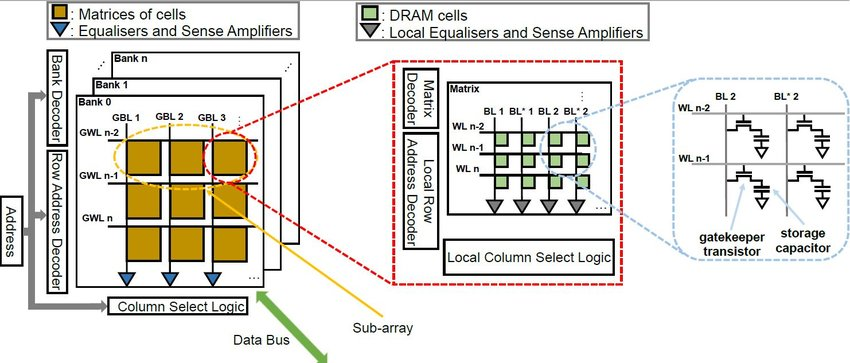
\includegraphics[scale=0.5]{estruturadram.png}
\centering
\caption{estrutra interna de uma \ac{DRAM}}
\label{imagem dram}
\end{figure}
\pagebreak

\subsection{Synchronous dynamic random-access memory}
\par \ac{SDRAM} é uma {DRAM} em que a operação do seu circuito no pino externo é coordenada por um \textit{clock signal}\footnote{sinal eletrónico digital que oscila entre um estado ligado e desligado a uma frequência constante.} externo. Existem ainda as \ac{DDR} que são uma classe das memórias do tipo \ac{SDRAM}. Distingue-se das restantes classes, que não serão abordadas neste relatório, uma vez que operam em \textit{double data rate}
\footnote{a transferência de dados ocorre em dois momentos, o primeiro na subida e o segundo na descida.}, no entanto o tempo de transmissão de dados não é o dobro, relativamente às memórias em operam em single data rate, uma vez que a primeira transmissão de dados possui um delay relativamente alto, não sendo possível compensar no segundo envio de dados, a sua velocidade, é no entanto deveras superior às que possuem o mecanismo de single data rate. Atualmente as \ac{DDR} encontram-se na quinta geração, com o nome de DDR5 SDRAM. As versões posteriores não são compatíveis com as versões anteriores, uma vez que a frequência dos circuitos não possui o mesmo valor.


\section{Static Random Access Memory}
\label{staticram}
\par Por outro lado, a \ac{SRAM} é um tipo de memória que armazena os dados em forma de bits desde que esteja a ser alimentada por uma fonte de energia constante. Ao contrário da \ac{DRAM}, esta memória não precisa de ser atualizada de forma contínua o que resulta numa performance mais elevada assim como numa maior eficiência energética. Por outro lado, o custo e o espaço ocupado num circuito computacional é maior. O uso de flip flops permite aos bits estarem ativos enquanto a energia está presente, possibilitando assim o acesso imediato à porção desejada sem que seja preciso percorrer sequencialmente toda a unidade, o que proporciona uma velocidade de escrita e leitura extremamente elevada.
\par O circuito utilizado é um circuito \textit{Flip-Flop} que tem apenas dois estados, desligado ou ligado, que são representados ,respetivamente, por 0 e 1. Ao contrário da \ac{DRAM} que apenas utiliza um capacitor e um transitor por célula de memória, a \ac{SRAM} utiliza 6 transitores, 2 para aceder à célula e 4 para armazenar dados. 
\par Através da análise da figura \ref{tabela sram dram} é possível observar as diferenças entre os dois tipos de memórias.
\begin{figure}
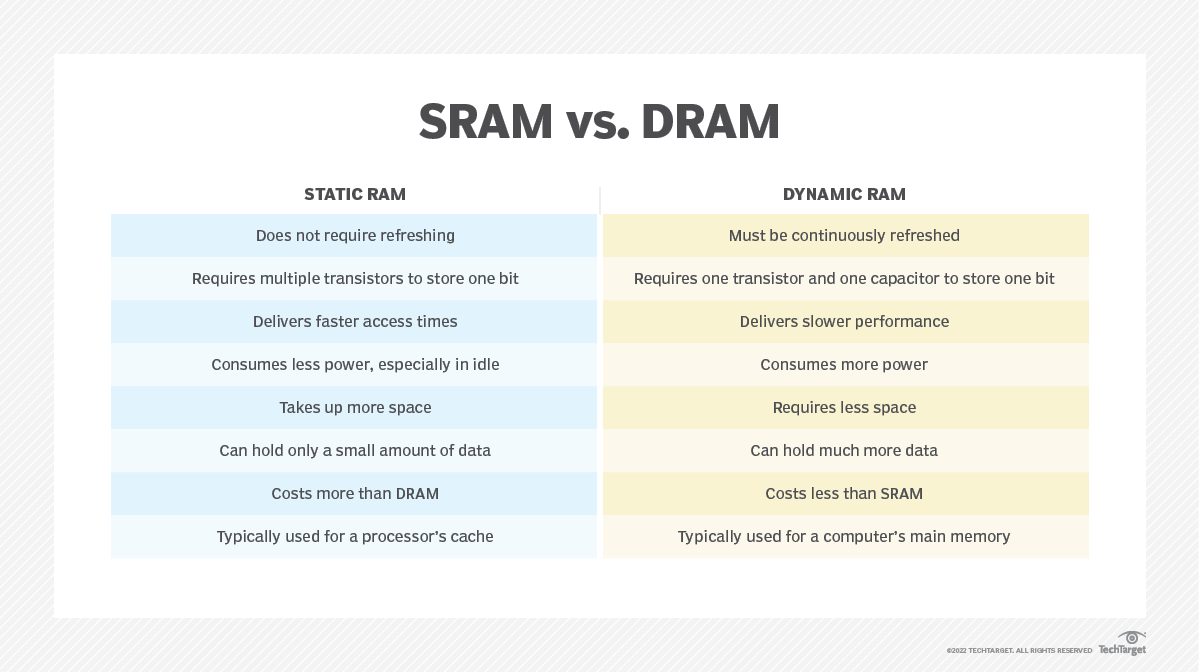
\includegraphics[scale=0.3]{dramsram.png}
\caption{Tabela de comparação entre \ac{SRAM} e \ac{DRAM}}
\label{tabela sram dram}
\end{figure}
\pagebreak

\subsection{Memória Cache}
\label{cache}
\par A memória cache\footnote{local onde os dados que necessitam de ser acedidos frequentemente são guardados} é uma memória de acesso rápido, do tipo \ac{SRAM} que é utilizada pelos processadores e que tem como objetivo reduzir o tempo de demora no acesso aos dados armazenados pela memória. A quantidade de dados que consegue armazenar é deveras reduzida, no entanto a sua velocidade é altíssima.
\subsubsection{Cache L1}
\label{cache l1}
\par A capacidade de processamento de um \ac{Cpu} é muito superior à da memória \ac{RAM}, por este motivo a memória cache é dividada em 3 tipos, L1, L2 e L3. Este primeiro opera numa frequência muito perta da do processador e, por isso, encontra-se alocado muito perto deste, no entanto esta frequência não é imediatamente atingida, sendo necessários alguns ciclos de clock para tal ser atingido. São apenas utilizados até 256 KB deste tipo de memória. Este encontra-se dividido em duas partes, uma para aceder a dados e outra para instruções. A sua velocidade máxima é de 1150 GB/s. Cada núcelo do processador possui a sua própria memória L1, ou seja, um processador com 10 cores, possui 10 unidades de Cache do tipo L1. 
\subsubsection{Cache L2}
\label{cache l2}
\par Por outro lado, o Cache L2 nao possui uma velocidade nem largura de banda tão elevadas como o Cache L1, possui no entanto menos transitores o que permite que o seu custo de fabrico e por consequência de venda seja menor, sendo assim usado em maior quantidade. O seu uso é variado, mas começa nos 256 KB, apesarem de serem bastante poucos os processadores que usem tão pouca quantidade, e podem chegar a ter 15 MB nos modelos com um custo mais elevado. A sua velocidade máxima é de 470 GB/s. Ao contrário do anterior, este não se encontra dividido em duas porções e podem, ou não, compartilhar a unidade com outros cores, nos processadores de gama alta tal não acontece, sendo uma unidade de cache L2, exclusiva para um core.
\subsubsection{Cache L3}
\label {cache l3}
\par Por fim, a memória cache com menor velocidade é o L3, com uma velocidade máxima de 200 GB/s, no entanto é aquela que é usada em maior quantidade, sendo utilizados até 64 MB. É no entanto compartilhada pelos vários núcelos do processador, sendo, normalmente, a quantidade de armazenamento divida de forma igual entre os núcelos do processador.
\pagebreak



\section{Virtual Random access Memory}
\par Com a evolução dos ambientes gráficos, nomeadamente a parte das cores, onde houve um aumento significativo do número de cores disponíveis para serem exibidas num dispositivo capaz de o fazer foi necessário criar uma variante da \ac{RAM} que se dedicasse ao processamento de imagem gráfica. A sua estrutura foi concebida de maneira a que seja possível o acesso em simultâneo por parte do \ac{GPU} e do monitor. Tal só é possível através do uso de bancos de dados dentro da memória, onde várias células estão a ser utilizadas para leitura ou escrita em simultâneo.

\par Encontra-se alojada no \ac{GPU} do dispositivo e é responsável por guardar a informação que este necessita para mostrar uma imagem no monitor. Esta memória mantém os dados necessários para formar uma imagem com taxas de frames por segundo constantes, de modo a proporcionar ao utilizador uma experiência agradável e fluida.

\par O \ac{Cpu} é responsável por fazer todos os cálculos e envia as informações para o \ac{GPU}, que ao ler essas informações, guarda-as na \ac{VRAM} que depois serão utilizadas por outras estruturas de modo a gerar uma imagem.
\par Para um uso, dito comum, a \ac{VRAM} é pouco utilizada, mas mesmo assim não é dispensável, no entanto, o que realmente necessita de quantidades altas de \ac{VRAM} são os videojogos, o manipulamento tanto de imagem como de vídeo e para realizar modelação 3D. Na figura \ref{foto_vram} é possível verificar a alocação da \ac{VRAM}
\begin{figure}[h]
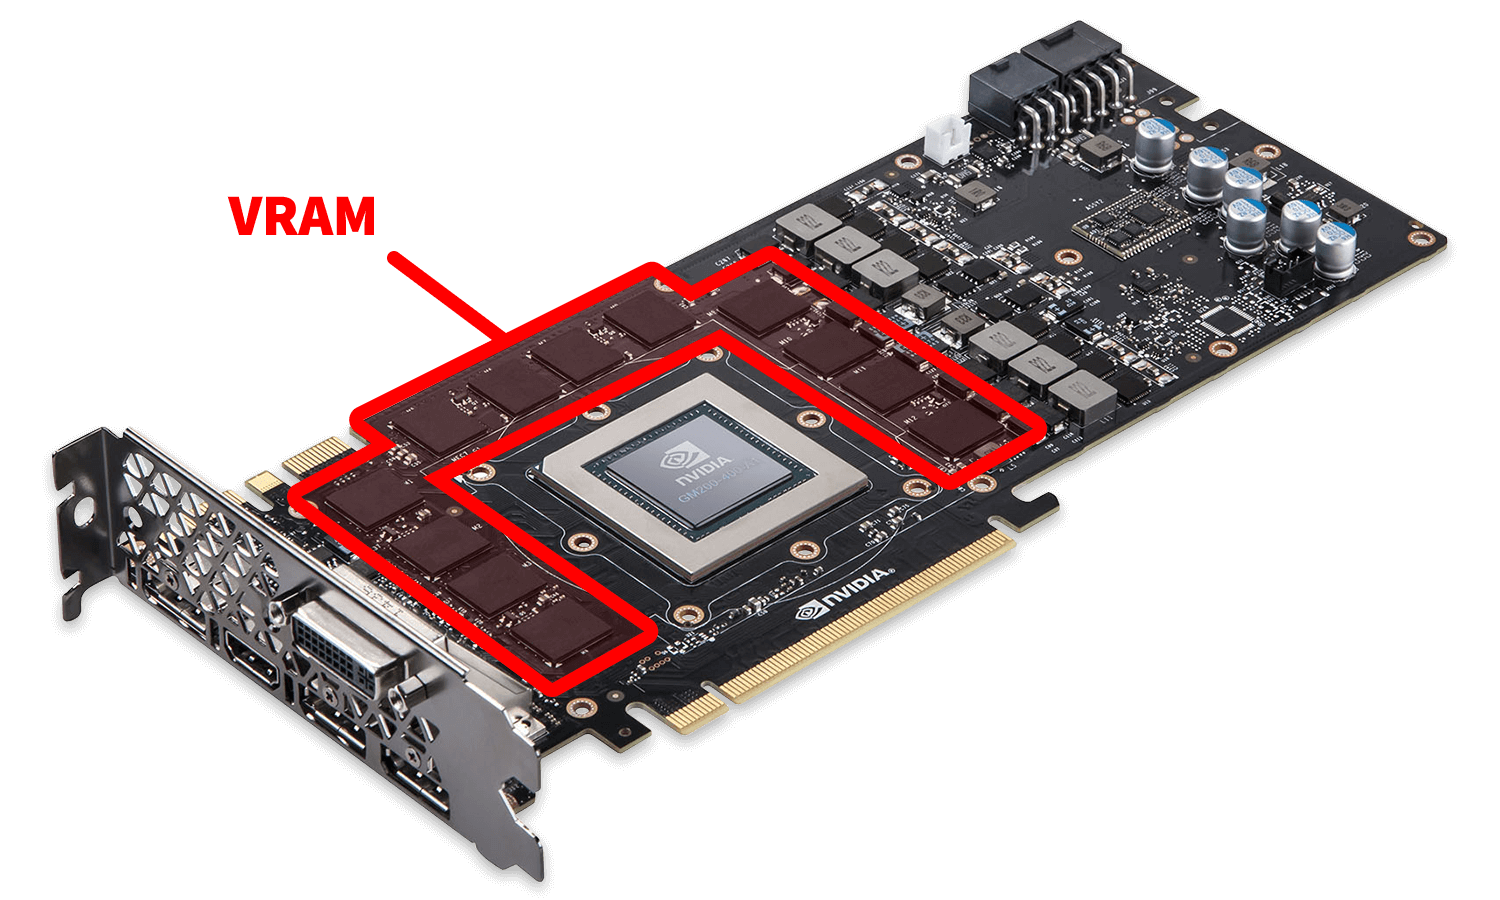
\includegraphics[scale=0.1]{vram_152.png}
\caption{Placa de vídeo}
\label{foto_vram}
\end{figure}


\subsection{Window Dynamic Random Access Memory}


\par Antes do surgimento e o uso mainstream de \ac{DDR} e \ac{VRAM}, \ac{WRAM} era um tipo de memória utilizada frequentemente em placas de vídeo entre a década de 1990 e o início dos anos 2000. A principal característica da \ac{WRAM} era a operação de escrita e leitura em simultâneo, em diferentes áreas da memória, denominadas de \textit{janelas\textbackslash windows} e daí o nome desta variante de \ac{RAM}. Esta diferença melhorava em grande escala a largura de banda permitida à placa de vídeo acelerando a transferência de dados e, finalmente, melhorando o desempenho gráfico do mesmo componente.






\chapter{Aplicações práticas}
\par Dados os conceitos sobre os vários tipos de memórias, é possível agora explicar as aplicações práticas destas de uma forma mais técnica e objetiva.
\par Começando pela \ac{SRAM}, esta é principalmente utilizada para armazenar dados cache do processador devido à sua altíssima velocidade, estabilidade energética, capacidade de reter os dados atráves de uma única fonte de alimentação constante permitindo ter um maior controlo sobre a memória, uma vez, que não está dependente de ciclos de atualização e ainda baixo consumo de energia e maior precisão no acesso aos dados já armazenados. É também utilizada em microprocessadores onde a alta velocidade é necessária, mas aonde a energia disponível é também ela baixa. O que torna esta memória ideal para as utilizações descritas é o facto de esta não ter limitações ao nível de ciclos de escrita\textbackslash leitura, o que a torna ideal para aplicações que registam dados em tempo real. Para além do elevado custo, estas possuem uma dimensão também elevada e não possuem a capacidade de armazenar grandes quantidades de dados pelo que o seu uso em situações onde é necessário o armazenamento de uma quantidade elevada de dados para serem acessados de modo imediato torna-se inviável, sendo no entanto possível mas, como já referido anteriormente, acarreta um custo elevado, de aproximadamente 8 vezes por bit em relação às \ac{DRAM}.

\par Por outro lado, a \ac{DRAM} é utilizada para fins onde a alta velocidade não é a prioridade mas sim, onde é necessário um armazenamento mais económico para grandes quantidades de dados. É então utilizada como memória principal em Desktops e Laptops, consolas de videojogos e \ac{GPU}s sob a forma de \ac{VRAM}. É também utilizada em grandes servidores onde é necessário o uso de \ac{RAM} de forma extensiva, sendo por isso preferida sobre a \ac{SRAM} devido ao baixo custo e alta eficiencia que apresenta. O baixo custo da \ac{DRAM} apenas é possível, uma vez que, cada bit apenas é necessário um transitor e um capacitor, ao contrário do que acontece nas \ac{SRAM}, como já foi referido no subcapítulo \ref{staticram}.
\label{chap.aplicacoes}




\chapter{Evolução ao longo dos anos}
\label{chap.evolução}
\section{As primeiras Formas de Ram}
\label{Primeira ram}

\par Nos primórdios da computação, para efeitos de memória, eram utilizados contadores mecânicos e linhas de atraso. Como se tratavam de processos mecânicos, a sua leitura era apenas possível de ser feita através de modo sequêncial. No caso das memórias tambor, era necessário ter conhecimento do layout físico da memória de forma a recuperar dados que haviam sido escritos anteriormente.

\begin{figure}[b]
\includegraphics[scale=0.5]{tubo.jpg}
\caption{Cathode Ray tube}
\label{crt}
\end{figure}

\par A primeira forma de \ac{RAM} apareceu em 1947, com o nome de de Williams tube, criado e desenvolvido por Freddie Williams e Tom Kilburn, os dados eram armazenados na forma de pontos eletricamente carregados na face de um tubo de raios catódicos, figura \ref{crt}. O funcionamento do tubo consistia nos pontos eletricamente carregados apagarem aqueles que estavam diretamente ao seu lado, devido a estarem descompensados a nível elétrico, deste modo uma sequência de pontos carregados eletricamente na horizontal apagaria aquele ao seu lado e assim sucessivamente, este processo representava uma palavra no computador, caso a energia do feixe que atravessa o tubo fosse aumentada, a palavra tornar-se-ia maior e mais nítida, mas mais afastada, pois os pontos carregados iriam apagar os do lado devido ao aumento da carga neles exercida.  Como o feixe de eletrões podia escrever e ler os pontos do tubo em qualquer ordem, estava então criada a primeira memória da acesso aleatório, \ac{RAM}. Continha, no entanto, algumas limitações, como o facto de o feixe de energia ter de ser suficientemente grande para produzir pontos que apresentassem um tempo de vida útil aproveitável, a memória tinha e então um limite na sua densidade, o que significava que eram apenas possíveis armazenar no máximo, 2560 bits de dados.

\section{Memória de Núcleo magnético}


\par A memória de núcleo magnético foi criada em 1947 e desenvolvida até meados da década de 1970. O seu funcionamento consiste em cores, juntos entre si, sobre a forma de camadas com os fios que os ligam, a passarem no orifício presente no centro dos cores, sendo que por cada orifício passam 2 ou mais fios. E assim como a tendência de um circuito magnético é a preservação do estado atual, isto permitia que os cores armazenassem o seu estado, que poderia ser ~ligado ou desligado. Quando a energia era suprimida, os cores mantinha a sua informação, não sendo assim considerados uma \ac{RAM}, mas os avanços tecnológicos obtidos através do desenvolvimento deste tipo de armazenamento foram essenciais para o desenvolvimento das \ac{RAM}s, tendo então sido aqui mencionado.
\subsection{Magnetoresistive Random Access Memory}
\par \ac{MRAM} ao contrário da grande maioria das memórias apresentadas neste documento é um tipo de memória não volátil que utiliza propriedades magnéticas para armazenar os dados, diferenciando-se das outras memórias com o facto que não perder os dados registados quando deixa de receber energia. A \ac{MRAM} armazena dados através de um processo denominado de magnetorresistência, onde a resistência provocada por um material magnético pode variar dependendo do campo magnético ao qual este é exposto, permitindo assim que os dados sejam armazenados como orientações magnéticas.
\par O aparecimento da \ac{MRAM} remete para a década de 1980 quando investigadores começaram a exploração do potencial do efeito de magnetorresistência, no entanto o seu surgimento é colocado na primeira década de 2000. A \ac{MRAM} oferecia alta densidade, baixo consumo, acesso rápido e capacidade de reter dados na possibilidade de falta de energia, sendo portanto uma possibilidade interessante para por exemplo armazenamento apesar de enfrentar grandes competidores de armazenamento como NAND Flash e \ac{DRAM}.

\section{As memórias utilizadas atualmente}
\subsection{Evolução da \ac{DRAM}}


\par A \ac{DRAM} surgiu durante a segunda Guerra Mundial, sendo o primeiro conceito oficial desenvolvido em 1966 por Robert Dennard enquanto trabalhava na IBM. O primeiro chip de memória \ac{DRAM} foi lançado em meados dos anos 1970, embora mais lento que tecnologias anteriores como a que vamos referir no seguinte paragrafo, provou o seu valor com o grande avanço de capacidade de armazenamento de dados e ao seu baixo custo por bit em comparação com as demais alternativas existentes na época, tornando-se muito rapidamente a forma dominante de memória de acesso aleatório mais usada em computadores e dispositivos eletrônicos. Ao longo das décadas, novas e melhores versões desta memória surgiram tais como: \ac{FPM}, \ac{EDO}, \ac{SDRAM} e \ac{DDR}.

\subsection{Evolução da \ac{SRAM}}

\par A \ac{SRAM} surgiu em 1963 desenvolvida por Robert Norman enquanto trabalhava na Fairchild Semiconductor. Empresas líderes de mercado tais como a IBM, Intel, etc, foram pioneiras no desenvolvimento desta tecnologia. Esta tornou-se crucial para o desenvolvimento de dispositivos que necessitavam de frequente uso de cache em processadores e em contextos nos quais a velocidade de acesso era crucial.

\subsection{Evolução da \ac{VRAM}}

\par No caso da \ac{VRAM} a invenção e desenvolvimento da mesma não pode ser atribuída a um único criador, mas sim a um longo processo de mútua colaboração entre várias empresas e engenheiros da indústria tecnológica. A sua primeira introdução ocorreu no início dos anos 80, sendo algumas das mais influentes empresas participantes no desenvolvimento da mesma sendo estas a IBM e a Fujitsu e Hitachi. Entre os vários tipos de \ac{VRAM} desenvolvidos ao longo dos anos. Um dos primeiros tipos foi a \ac{VRAM} Estática, similarmente surgiu a \ac{VRAM} Dinâmica que apesar de não ser tão rápida como a anterior era significativamente mais densa. Agora alguns tipos de \ac{VRAM} mais recentes são: \ac{GDDR} usada de forma extensiva em placas de vídeo, um dos componentes mais relevantes num computador ou dispositivo que apresente inferface gráfica, sendo que este já possui várias gerações com várias inovações, sendo a mais relevante a velocidade. Ordenando por ordem cronológica temos então: \ac{GDDR}, \ac{GDDR}2, \ac{GDDR}3, \ac{GDDR}4, \ac{GDDR}5, \ac{GDDR}6 e \ac{GDDR}6X. Ainda outro tipo que poderia ser abordado seria a \ac{HBM}, um tipo de memória de diferente construção e com um diferente propósito e, portanto, sendo usada em fins diferente de GDDR, sendo a sua evolução dada de maneira cronológica por: \ac{HBM}, \ac{HBM}2, e \ac{HBM}3.

\subsection{Surgimento da \ac{SDRAM}}

\par Atualmente o tipo de \ac{RAM} mais utilizado é a \ac{SDRAM} sendo uma evolução da \ac{DRAM} convencional. A primeira geração de \ac{SDRAM} surgiu por volta dos anos 1990, esta nova tecnologia oferecia vastas vantagens e inovações em comparação com a \ac{DRAM} tradicional. De modo similar à \ac{VRAM}, a criação da mesma não pode ser associada a uma única entidade, mas à combinação de esforços das empresas líderes de mercado, tais como a Samsung, Micron e Hynix. A \ac{SRAM} DDR já se encontra na sua quinta geração sendo os seus precedentes, DDR, DDR2, DDR3, DDR4 e DDR5. Em cada geração houve melhorias exponenciais na largura de banda, na densidade do componente, na eficiência energética e na velocidade de leitura e escrita de dados. Como consequência da DDR5 ser ainda bastante recente, o custo deste componente é elevado, sendo por isso a DDR4 a líder de mercado nesta categoria.



\chapter{Atualidade e prespetivas para o futuro}
\label{chap.atualidade}
\section{Ponto Crítico da \ac{SRAM} e possíveis soluções}

\par A evolução da \ac{SRAM} está a atingir um ponto crítico, os limites da física, isto porque de modo a aumentar a velocidade é necessário aumentar a densidade, de forma ao espaço percorrido pelos sinais ser menor, contudo os materiais possuem um limite quanto a este aspeto, deste modo, atualmente existem equipas de investigadores a trabalharem numa maneira de poderem aumentar ainda mais a densidade, sendo que um dos desenvolvimentos passa pelo procura de um material que consiga suportar maiores densidades. Uma tecnologia que está em desenvolvimento e apresenta um futuro promissor, no entanto sem qualquer certeza, são memórias baseadas em nanotubos de carbono.
\par Atualmente as \ac{SRAM}s continuam a ser uma peça fundamental em qualquer sistema computacional devido às velocidades de acesso extremamente elevadas, expecialmente em dispositivos de alta performance, incentivando assim a inovação para a resolução dos problemas que atualmente enfrenta.

\section{Ponto Crítico da \ac{DRAM} e possíveis soluções}


\par A geração atual de \ac{DDR} denomina-se por, DDR5 SDRAM, foi desenvolvida inicialmente em 2017 pela coorporativa \textit{Joint Electron Device Engineering Council}, apoiada pelos maiores vendedores e desenvolvedores de memórias. Em relação há geração anterior verificou-se um aumento de 50\% na largura de banda. A geração anterior tinha um teto de 3200MT/s\footnote{Megatransfers per second}, enquanto que a nova geração começa nos 4800Mt/s e pode tem uma teto de 6400MT/s.
\par Para o futuro, as \ac{DRAM} enfrentam adversidades bastante semelhantes às que as \ac{SRAM} enfrentam. De forma a resolver esses problemas, a indústria tem testado tecnologias em ascensão tais como memórias restritivas, memórias de mudança de fase e outras abordagens que passam por memórias não voláteis. Devido também ao uso extensivo desta memória, é do interesse da indústria a aposta no desenvolvimento de técnicas inovadoras que permitam contornar os desafios atuais.

\section{A \ac{VRAM} e as consequências da seu desenvolvimento}

\par Recentemente a \ac{VRAM} tem evoluido de forma significativa devido ao aumento da resolução de imagens e vídeos, mas também devido ao surgimento de novos jogos que necessitam de um uso extensivo e prolongado do \ac{GPU}, deste modo a indústria viu-se obrigada a incorporar uma maior quantidade de \ac{VRAM} de modo a conseguir acompanhar o avanço da resolução das imagens e vídeos, como consequência de tal facto, os editores tanto a nível de vídeo como de imagem, necessitam também de maior capacidade de processamento de imagem. A solução encontrada foi incorporar uma maior quantidade de \ac{VRAM} no \ac{GPU}.

\par No entanto, a solução para o futuro não passa apenas pela incorporação de uma maior quantidade de \ac{VRAM}, mas sim pelo aumento da capacidade deste tipo de memória, sendo este essencial para a evolução também da realidade virtual. Outro aspeto com igual notoriedade é o aumento da largura de banda e a efeciência energética, tais resultados iriam permitir reduzir de forma significativa as quebras de performance que acontecem atualmente devido ao uso extensivo da \ac{VRAM}.

\par Esta evolução irá permitir expandir os horizontes no campo da  realidade virtual permitindo assim uma experiência totalmente imersiva neste campo permitindo assim expandir os limites que este campo atualmente enfrenta. Mas não se resume apenas à realidade virtual, os dispositivos móveis seriam capazes de lidar com  gráficos ainda mais complexos permitindo assim uma experiência ainda mais imersiva neste tipo de dispositivos.

\chapter{Conclusões}
\label{chap.conclusão}
\par Após uma cuidada análise da informação recolhida e elaboração deste documento, foi possível chegar à conclusão que as memórias \ac{RAM} podem estar a chegar ao seu limite físico e que de modo a ser possível continuar o seu desenvolvimento serão necessários novos materias que consigam aumentar ainda mais a sua densidade.



\chapter*{Contribuições dos autores}
\par Cada autor contribuiu de maneira igual para a realização do trabalho pelo que é justo atribuir 50\% a cada um.
\par O resumo, capítulo 1 e Capítulo 6 foi realizado em conjunto
\par O TV realizou o 2 e 3 Capítulo
\par O PL realizou o Capítulo 4 e 5.
\vspace{10pt}


Pl Tv : 50\%, 50\%\\

%%%%%%%%%%%%%%%%%%%%%%%%%%%%%%%%%
\chapter*{Acrónimos}
\begin{acronym}
\acro{ua}[UA]{Universidade de Aveiro}
\acro{leci}[LECI]{Licenciatura em Engenharia de Computadores e Informática}
\acro{glisc}[GLISC]{Grey Literature International Steering Committee}
\acro{RAM}[RAM]{Random Access Memory}
\acro{GPU}[GPU]{Graphics Processor Unit}
\acro{VRAM}[VRAM]{Virtual Random Acess Memory}
\acro{DRAM}[DRAM]{Dynamic Random Acess Memory}
\acro{Cpu}[Cpu]{Central processing unit}
\acro{Ssd}[Ssd]{Solid State Drive}
\acro{SRAM}[SRAM]{Static Random Acess Memory}
\acro{SDRAM}[SDRAM]{Synchronous dynamic random-access memory}
\acro{DDR}[DDR SDRAM]{Double Data Rate Synchronous Dynamic Random Access Memory}
\acro{FPM}[FPM]{Faste Page Mode}
\acro{EDO}[EDO]{Extended Data Out}
\acro{GDDR}[GDDR]{Graphics Double Data Rate}
\acro{HBM}[HBM]{High Bandwith Memory}
\acro{MRAM}[MRAM]{Magneto-resistive Random Access Memory}
\acro{WRAM}[WRAM]{Window Dynamic Random Access Memory}
\end{acronym}


%%%%%%%%%%%%%%%%%%%%%%%%%%%%%%%%%
\printbibliography

\end{document}
